\documentclass[watermark,twoside]{favf-thesis}
	% default language English

\usepackage{xspace}
\usepackage{amsmath}
\usepackage{amsfonts}
\usepackage{amssymb}
\usepackage{bm}
\usepackage{upgreek}
\usepackage{graphicx}
\usepackage{ifthen}


\newcommand{\latex}{\LaTeX\xspace}


%%%%%%%%%%%%%%%%
%              %
%  references  %
%              %
%%%%%%%%%%%%%%%%

\newcommand{\reffig}[1]{Figure~\ref{fig:#1}}
\newcommand{\refsubfig}[1]{Figure~\ref{subfig:#1}}


%%%%%%%%%%
%        %
%  sets  %
%        %
%%%%%%%%%%


\newcommand{\setN}{\ensuremath{\mathbb{N}}}  % natural numbers
\newcommand{\setZ}{\ensuremath{\mathbb{Z}}}  % integers
\newcommand{\setQ}{\ensuremath{\mathbb{Q}}}  % rational numbers
\newcommand{\setR}{\ensuremath{\mathbb{R}}}  % reals
\newcommand{\setC}{\ensuremath{\mathbb{C}}}  % complex numbers



%%%%%%%%%%%%%%%%%%%%%%%%%%%%%
%                           %
%  formatting of variables  %
%                           %
%%%%%%%%%%%%%%%%%%%%%%%%%%%%%

% variable:
\newcommand{\var}[1]{\ensuremath{#1}}

% complex variable:
\newcommand{\cvar}[1]{\ensuremath{\underline{#1}\,}}

% vectors
\renewcommand{\vec}[1]{\ensuremath{\bm{#1}}}
\newcommand{\vecTr}[1]{\ensuremath{\bm{#1}\mTr}}
\newcommand{\vecHerm}[1]{\ensuremath{\bm{#1}}\mHerm}

\newcommand{\cvec}[1]{\vec{\cvar{#1}}}
\newcommand{\cvecTr}[1]{\vecTr{\cvar{#1}}}
\newcommand{\cvecHerm}[1]{\vecHerm{\cvar{#1}}}


% matrices
\newcommand{\mat}[1]{\vec{#1}}
\newcommand{\matTr}[1]{\vecTr{#1}}
\newcommand{\matHerm}[1]{\vecHerm{#1}}

\newcommand{\cmat}[1]{\cvec{#1}}
\newcommand{\cmatTr}[1]{\cvecTr{#1}}
\newcommand{\cmatHerm}[1]{\cvecHerm{#1}}



%%%%%%%%%%%%%%%%%%%%%%%%%%%%%
%                           %
%  formatting of functions  %
%                           %
%%%%%%%%%%%%%%%%%%%%%%%%%%%%%


\newcommand{\func}[1]{\ensuremath{\mathrm{#1}}}                          % function that returns a real-valued scalar
\newcommand{\cfunc}[1]{\ensuremath{\underline{\mathrm{#1}}\,}}           % function that returns a complex-valued scalar
\newcommand{\vecfunc}[1]{\ensuremath{\bm{\mathrm{#1}}}}                  % function that returns a real-valued vector
\newcommand{\cvecfunc}[1]{\ensuremath{\underline{\bm{\mathrm{#1}}}\,}}   % function that returns a complex-valued vector
\newcommand{\matfunc}[1]{\vecfunc{#1}}                                   % function that returns a real-valued matrix
\newcommand{\cmatfunc}[1]{\cvecfunc{#1}}                                 % function that returns a complex-valued scalar



%%%%%%%%%%%%%%%%%%%%%%%%%%%%%%%%%%%%%%
%                                    %
%  standard functions and operators  %
%                                    %
%%%%%%%%%%%%%%%%%%%%%%%%%%%%%%%%%%%%%%


% operators on complex numbers
\newcommand{\cConj}{\ensuremath{^\ast}}                                             % complex conjugate
\newcommand{\cReal}[1]{\ensuremath{\mathcal{R}\left\lbrace #1 \right\rbrace}}      % real part
\newcommand{\cImag}[1]{\ensuremath{\mathcal{I}\left\lbrace #1 \right\rbrace}}      % imaginary part


% unary matrix/vector operators (suffixes):
\newcommand{\mTr}{\ensuremath{^\mathrm{T}}}           % transposition
\newcommand{\mHerm}{\ensuremath{^\mathrm{H}}}         % Hermitian transpose (complex conjugate transpose)

\newcommand{\mInv}{\ensuremath{^{\text{-}1}}}                % matrix inverse
\newcommand{\mInvTr}{\ensuremath{^{-\mathrm{T}}}}     % transpose of matrix inverse
\newcommand{\mInvHerm}{\ensuremath{^{-\mathrm{H}}}}   % hermitian transpose of matrix inverse
\newcommand{\mPinv}{\ensuremath{^\text{\dag}}}            % Moore-Penrose pseudo-inverse

\newcommand{\matInv}[1]{\ensuremath{\mat{#1}\mInv}}
\newcommand{\cmatInv}[1]{\ensuremath{\cmat{#1}\mInv}}
\newcommand{\matPinv}[1]{\ensuremath{\mat{#1}\mPinv}}
\newcommand{\cmatPinv}[1]{\ensuremath{\cmat{#1}\mPinv}}


% binary matrix/vector operators:
\newcommand{\mKron}{\ensuremath{\otimes}}             % Kronecker product
\newcommand{\mKhatri}{\ensuremath{\diamond}}          % Khatri-Rao product
\newcommand{\mElemProd}{\ensuremath{\odot}}           % hadamard (element-wise) product


% other operators
\newcommand{\mNorm}[2]{\ensuremath{\left\| #1 \right\|_{#2}}}         % general norm
\newcommand{\mFrobNorm}[1]{\mNorm{#1}{\text{F}}}                      % Frobenius norm
\newcommand{\mDiag}[1]{\ensuremath{\mathrm{diag}\left(#1\right)}}     % for matrices: returns main diagonal as vector; for vecor: returns diagonal matrix
\newcommand{\mTrace}[1]{\ensuremath{\mathrm{trace}\left(#1\right)}}   % sum of diagonal elements
\newcommand{\mDet}[1]{\ensuremath{\mathrm{det}\left(#1\right)}}       % determinant



%%%%%%%%%%%%%%%%%
%               %
%  convolution  %
%               %
%%%%%%%%%%%%%%%%%

\makeatletter
\newcommand{\convolve}{\ensuremath{\ast}}
\newcommand{\circConvolve}{\ensuremath{\mathbin{\mathpalette\make@circled\ast}}}
\newcommand{\make@circled}[2]{%
  \ooalign{$\m@th#1\smallbigcirc{#1}$\cr\hidewidth$\m@th#1#2$\hidewidth\cr}%
}
\newcommand{\smallbigcirc}[1]{%
  \vcenter{\hbox{\scalebox{0.77778}{$\m@th#1\bigcirc$}}}%
}
\makeatother


%%%%%%%%%%%%%%%%%%%%%%%%
%                      %
%  coordinate systems  %
%                      %
%%%%%%%%%%%%%%%%%%%%%%%%

% azimuth angle:
\newcommand{\azi}{\ensuremath{\varphi}}
\newcommand{\upazi}{\ensuremath{\upvarphi}}  % non-italic

% elevation angle:
\newcommand{\ele}{\ensuremath{\vartheta}}
\newcommand{\upele}{\ensuremath{\upvartheta}}  % non-italic

% helper command for command \coele and  \upcoele (see below)
\newcommand{\hslashslash}{%
  \raisebox{.9ex}{%
    \scalebox{.7}{%
      \rotatebox[origin=c]{18}{$-$}%
    }%
  }%
}

% co-elevation:
%   - Ranges from positive y-axis (0°/0 rad) to negative y-axis (180°/? rad).
%   - Formatted using a \vartheta with a slash.
\DeclareRobustCommand{\coele}{%
  {% keep these braces!
    \ensuremath{%                            
    \vphantom{\vartheta}%
    \ooalign{\kern-.07em\smash{\lower.35em\hbox{\hslashslash}}\hidewidth\cr$\vartheta$\cr}%
    \kern.05em
    }%
  }%
}

% non-italic co-elevation
\newcommand{\upcoele}{%
  {% keep these braces!
    \text{% needed to scale correctly in subscripts
      \ensuremath{%
        \vphantom{\upvartheta}%
        \ooalign{\kern-.07em\smash{\lower.35em\hbox{\hslashslash}}\hidewidth\cr$\upvartheta$\cr}%
        \kern.05em%
      }%
    }%
  }%
}



%%%%%%%%%%%%%%%%%
%               %
%  derivatives  %
%               %
%%%%%%%%%%%%%%%%%

% differential 'd':
\newcommand{\diff}{\mathrm{d}}

% make \partial symbol upright:
\let\oldpartial\partial
\DeclareRobustCommand{\uppartial}{\text{\rotatebox[origin=t]{20}{\scalebox{0.95}[1]{$\oldpartial$}}}\hspace{-1pt}}
\renewcommand{\partial}{\uppartial}

\newcommand{\pDiff}{\uppartial} % alias (to be consistent with \diff)


\newcommand{\deriv}[3][]{%
  \ifthenelse{\equal {#1}{}}{% no order given:
    \frac{\diff #2}{\diff #3}%
  }{ % order given:
    \frac{\diff^{#1} #2}{\diff #3^{#1}}%
  }%
}

\newcommand{\pDeriv}[3][]{%
  \ifthenelse{\equal {#1}{}}{% no order given:
    \frac{\pDiff #2}{\partial #3}%
  }{% order given:
    \frac{\pDiff^{#1} #2}{\partial #3^{#1}}%
  }%
}



%%%%%%%%%%%%%%%%%%%%%%%%%%%%%%%%
%                              %
%  general transform commands  %
%                              %
%%%%%%%%%%%%%%%%%%%%%%%%%%%%%%%%

% based on package trfsgns (https://ctan.org/pkg/trfsigns):

% transform:
%
% #1: argument for the resulting function or series
% #2: letter or name of the transform
% #3: expression that is being transformed
% #4: subscript text (e.g., for giving the variable over which the transform in performed)
\newcommand{\mathTransform}[4]{%
  \ensuremath{%
      \operatorname*{#2}%
      \ifthenelse{\equal {#4}{}}{% no argument for subscript text        
      }{% argument for subscript text given
        _{#4} %
      }%
      \kern-2.0pt%
      \left\lbrace #3 \right\rbrace%
      \ifthenelse{\equal {#1}{}}{% no argument for resulting function given        
      }{% argument for resulting function given
        \kern-2.0pt #1 %
      }%
  }%
}


% continues transform
%
% #1: argument for the resulting function (example: F{g(t)}(f) <-- 'f' is the argument)
%     --> If not empty, the argument will be enclosed in round brackets.
% #2: letter or name of the transform
% #3: expression that is being transformed
\newcommand{\mathContTransform}[4]{%
  \mathTransform%
  { \if\relax\detokenize{#1}\relax\else\ensuremath{\left( #1 \right)}\fi }% enclose in round brackets if optional argument is given
  {#2}{#3}{#4}%
}

% discrete transform
%
% #1: argument for the resulting series (example: F{g[n]}[k] <-- 'k' is the argument)
%     --> If not empty, the argument will be enclosed in square brackets.
% #2: letter or name of the transform
% #3: expression that is being transformed
\newcommand{\mathDiscTransform}[4]{%
  \mathTransform%
  { \if\relax\detokenize{#1}\relax\else\ensuremath{\left[ #1 \right]}\fi }% enclose in square brackets if optional argument is given
  {#2}{#3}{#4}%
}

% inverse continues transform
%
% #1: argument for the resulting function (example: F^-1{g(f)}(t) <-- 't' is the argument)
%     --> If given, the argument will be enclosed in round brackets.
% #2: letter or name of the transform
% #3: expression that is being inverse-transformed
\newcommand{\mathContInvTransform}[4]{\mathContTransform{#1}{#2\mInv}{#3}{#4}}

% discrete inverse transform
%
% #1: argument for the resulting series (example: F^-1{g[n]}[k] <-- 'k' is the argument)
%     --> If given, the argument will be enclosed in square brackets.
% #2: letter or name of the transform
% #3: expression that is being inverse-transformed
\newcommand{\mathDiscInvTransform}[4]{\mathDiscTransform{#1}{#2\mInv}{#3}{#4}}


% Transform relation.
% --> Has a a hollow circle at the left and a solid cicle on the right, connected by a horizontal line.
%
% #1 (optional): Symbol for the transformation (written above the horizontal line)
\makeatletter
\newcommand{\transformRelation}[1][]{%
  \mathop{%
    \mbox{%
      \setlength{\unitlength}{0.1em}%
      \begin{picture}(37,10)%
        \put(4,3){\circle{4}}%
        \put(6,3){\line(1,0){26}}%
        \put(33,3){\circle*{4}}%
        \put(19,7){\makebox(0,0){#1}}%
      \end{picture}%
    }%
  }\slimits@%
}
\makeatother


% Reversed transform relation.
% --> Like \transformRelation but with the solid circle at the left and the hollow circle at the right
%
% #1: Symbol for the transformation (written above the horizontal line)
\makeatletter
\newcommand{\revTransformRelation}[1][]{%
  \mathop{%
    \mbox{%
      \setlength{\unitlength}{0.1em}%
      \begin{picture}(37,10)%
        \put(4,3){\circle*{4}}%
        \put(6,3){\line(1,0){25}}%
        \put(33,3){\circle{4}}%
        \put(19,7){\makebox(0,0){#1}}%
      \end{picture}%
    }%
  }\slimits@%
}
\makeatother

% Create a continuous transform
%
% This will create commands \<name>Transform, \<name>InvTransform,
% \<name>Relation, and \<name>RevRelation, where <name> is the name
% of the transform.
%
% #1: name of the transform ('fourier', 'dft', 'laplace', ...)
% #2: Symbol/text used for the transform
\newcommand{\createContinuousTransform}[2]{%
%
  % create command \<#1>Transformation
  \expandafter\NewDocumentCommand\csname#1Transform\endcsname{E{_}{\relax}O{}m}{%
    \mathContTransform{##2}{#2}{##3}{##1}%
  }%
%
  % create command \<#1>InvTransformation
  \expandafter\NewDocumentCommand\csname#1InvTransform\endcsname{E{_}{\relax}O{}m}{%
    \mathContInvTransform{##2}{#2}{##3}{##1}%
  }%
%
  % create command \<#1>Relation
  \expandafter\newcommand\csname#1Relation\endcsname{%
    \mathop{\transformRelation[#2]{}}
  }%
%
  % create command \<#1>RevRelation
  \expandafter\newcommand\csname#1RevRelation\endcsname{%
    \mathop{\revTransformRelation[#2]{}}
  }%
}

% Create a discrete transform
%
% This will create commands \<name>Transform, \<name>InvTransform,
% \<name>Relation, and \<name>RevRelation, where <name> is the name
% of the transform.
%
% #1: name of the transform ('fourier', 'dft', 'laplace', ...)
% #2: Symbol/text used for the transform
\newcommand{\createDiscreteTransform}[2]{%
%
  % create command \<#1>Transformation
  % \expandafter\newcommand\csname#1Transform\endcsname[2][]{%
  \expandafter\NewDocumentCommand\csname#1Transform\endcsname{E{_}{\relax}O{}m}{%
    \mathDiscTransform{##2}{#2}{##3}{##1}%
  }%
%
  % create command \<#1>InvTransformation
  \expandafter\NewDocumentCommand\csname#1InvTransform\endcsname{E{_}{\relax}O{}m}{%
    \mathDiscInvTransform{##2}{#2}{##3}{##1}%
  }%
%
  % create command \<#1>Relation
  \expandafter\newcommand\csname#1Relation\endcsname{%
    \mathop{\transformRelation[#2]{}}
  }%
%
  % create command \<#1>RevRelation
  \expandafter\newcommand\csname#1RevRelation\endcsname{%
    \mathop{\revTransformRelation[#2]{}}
  }%
}


%%%%%%%%%%%%%%%%%%%%%%%%%
%                       %
%  specific transforms  %
%                       %
%%%%%%%%%%%%%%%%%%%%%%%%%


%% Fourier transform %%

% letter for the Fourier transform:
\newcommand{\fourierLetter}{\ensuremath{\mathcal{F}}}

% Create command:
%  \fourierTransform, \fourierInvTransform, \fourierRelation, \fourierRevRelation
\createContinuousTransform{fourier}{\fourierLetter}


%% Discrete Fourier transform %%

% letter for the Fourier transform:
\newcommand{\dftLetters}{\ensuremath{\mathcal{DFT}}}

% Create command:
%  \dftTransform, \dftInvTransform, \dftRelation, \dftRevRelation
\createDiscreteTransform{dft}{\dftLetters}


%% Laplace transform %%

% letter for the Laplace transform:
\newcommand{\laplaceLetter}{\ensuremath{\mathcal{L}}}

% Create command:
%  \laplaceTransform, \laplaceInvTransform, \laplaceRelation, \laplaceRevRelation
\createContinuousTransform{laplace}{\laplaceLetter}



%%%%%%%%%%%%%%%%%
%               %
%  stochastics  %
%               %
%%%%%%%%%%%%%%%%%

\NewDocumentCommand\expValue{e{_}m}{%
    \operatorname*{\mathbb{E}}\IfNoValueF{#1}{_{#1}} \left\lbrace #2 \right\rbrace%
}

\NewDocumentCommand\variance{e{_}m}{%
    \operatorname*{\mathrm{var}}\IfNoValueF{#1}{_{#1}} \left\lbrace #2 \right\rbrace%
}

\NewDocumentCommand\covariance{e{_}m}{%
    \operatorname*{\mathrm{cov}}\IfNoValueF{#1}{_{#1}} \left\lbrace #2 \right\rbrace%
}

\NewDocumentCommand\correlation{e{_}m}{%
    \operatorname*{\mathrm{corr}}\IfNoValueF{#1}{_{#1}} \left\lbrace #2 \right\rbrace%
}

\newcommand{\mCorr}[1]{\ensuremath{\mat{R}_{#1}}}
\newcommand{\mcCorr}[1]{\ensuremath{\cmat{R}_{#1}}}
\newcommand{\mCov}[1]{\ensuremath{\mat{C}_{#1}}}
\newcommand{\mcCov}[1]{\ensuremath{\cmat{C}_{#1}}}


%---------------------------------------- Additional Packages ------------------------------
\usepackage[export]{adjustbox}
\usepackage{acronym}
\usepackage{todonotes}
\usepackage{tabularx}
\usepackage[utf8]{inputenc}
\usepackage{comment}
\usepackage[flushmargin]{footmisc} % Deaktiviert das Einrücken
\usepackage{pdfpages}
\usepackage{subcaption}
\usepackage{array}
\usepackage{enumitem}
\usepackage{graphicx}
\usepackage{listings}
\usepackage{xcolor}
\usepackage{hyperref}
\usepackage{appendix}
\usepackage{multibib}


\newcommand{\quotemarks}[1]{\glqq#1\grqq}



%---------------------------------------- Variables ----------------------------------------

\author{Le Vi Nguyen}
\thesistype{Transferarbeit}
\thesiscite{Transferarbeit}
\title{Optimization of an IoT Infrastructure and RFID solution}
\hypersetup{hidelinks}

%---------------------------------------- Document generation ------------------------------
\definecolor{dkgreen}{rgb}{0,0.6,0}
\definecolor{gray}{rgb}{0.5,0.5,0.5}
\definecolor{mauve}{rgb}{0.58,0,0.82}
\definecolor{backcolour}{rgb}{0.98, 0.98, 0.95}

\lstset{frame=none,
  language=Python,
  aboveskip=3mm,
  belowskip=3mm,
  showstringspaces=false,
  columns=flexible,
  basicstyle={\small\ttfamily},
  numbers=left,
  backgroundcolor=\color{backcolour},
  numberstyle=\tiny\color{gray},
  keywordstyle=\color{blue},
  commentstyle=\color{dkgreen},
  stringstyle=\color{mauve},
  breaklines=true,
  breakatwhitespace=true,
  tabsize=3
}


\let\cleardoublepage\clearpage
\newcites{intern}{Quellenverzeichnis}

\begin{document}

% Change your name and the title of the thesis in the file 'titlepage'.
% Change your name and the title of the thesis here.
\newcommand{\saauthor}{Autorin} %Name of Student
\newcommand{\matrikel}{1000 7222 2497}
\newcommand{\sathema}{Prozessanalyse und Erstmodellierung des MDV-Ablaufs mittels Signavio}

% Research group head 
\newcommand{\saprof}{Dr.-Ing. Peter Schupp}

% Name the researcher who supervised you. If you had more than one supervisor, you can add a second one.
\newcommand{\sabetreuer}{Name of supervisor} 
%\newcommand{\sabetreuerb}{Name of second supervisor}


%---------------------------------------- Page generation ----------------------------------

% Everything below this line has to be left unchanged. Please do not alter!
\begin{titlepage}

% Logos auf gleicher Höhe links und rechts
\noindent
\begin{minipage}[t]{0.5\textwidth}

\includegraphics[scale=0.8]{images/steinbeis.png}
\end{minipage}
\hfill
\begin{minipage}[t]{0.45\textwidth}
\flushright

\includegraphics[scale=0.17]{images/AMG_logo.png}
\end{minipage}

\vspace{0.2cm}
\hrule

\vspace{1cm}

\begin{center}
{\Large \textsc{STEINBEIS-HOCHSCHULE}}\\
{\Large \textsc{SCHOOL OF MANAGEMENT AND TECHNOLOGY}}\\
\vspace{0.5cm}

{\large Studiengang Wirtschaftsingenieurwesen WING\_$11$}\\
{\large Fachgebiet Prozessmanagement und Prozessautomation PPR-01}\\

\vspace{1cm}

{\large Transferarbeit} \\ 
\vspace{2cm}
{\LARGE \normalfont\bfseries \sathema} \\
\vspace{2cm}
Eingereicht von: \\ 
Le Vi Nguyen \\

{\large Matrikelnummer \matrikel}
\vspace{1cm}

Betreuender Hochschullehrer: \\
{\large \saprof} \\
\vspace{1cm}
Betreuende Mitarbeitende Mercedes-AMG GmbH:\\ Nicole Günter

%{\large \sabetreuerb} \\
\vspace{1cm}
\selectlanguage{ngerman}
\today
\end{center}

\end{titlepage}

\pagenumbering{roman}

\chapter*{Eigenständigkeitserklärung}
\input{eigenständigkeitserklärung}

\acresetall
\tableofcontents
\clearpage


% List of acronyms. Add new/more acronyms in the corresponding file.
% Anhang (das sind dann Seiten von Daten bspw.) vielleicht hinzufügen und Listings Code
\chapter*{Abkürzungsverzeichnis}

\addcontentsline{toc}{chapter}{Abkürzungsverzeichnis}
\begin{acronym}[AAAAAAAAAAAAA]
    \acro{CoP}{Conformity of Production}
    \acro{ICE}{Internal Combustion Engine}
    \acro{MDV}{Manufacturer’s Declared Value}
    \acro{QFE}{Qualitätsfreigabe Emission und Verbrauch}
    \acro{SCM}{Supply-Chain-Management}
    \acro{WLTP}{Worldwide Harmonised Light-Duty Vehicles Test Procedure}
\end{acronym}
\clearpage

% List of figures. The list is generated automatically.
\addcontentsline{toc}{chapter}{\listfigurename}
\listoffigures
\clearpage


\pagenumbering{arabic}

% Includes all chapters of the thesis. You can add more chapters if required.
\chapter{Einleitung}
In vielen Unternehmen entstehen Abläufe zunächst aus praktischer Notwendigkeit heraus, ohne dass sie von Anfang an systematisch dokumentiert oder modelliert werden \cite{Pospiech2014}. Solches informelles Vorgehen stößt jedoch an seine Grenzen, wenn die Komplexität zunimmt, die Anzahl der beteiligten Fachbereiche wächst und die Anforderungen an die Nachvollziehbarkeit steigen. Genau in dieser Lage befindet sich der Prozess Manufacture's Declared Value \acs{MDV} Verbrauch und Reichweite bei Mercedes-AMG. Obwohl an diesem Prozess verschiedene Fachbereiche wie Entwicklung, Zertifizierung und Vertrieb beteiligt sind und regulatorische Anforderungen eine hohe Verlässlichkeit verlangen, liegt bislang kein dokumentiertes oder modelliertes Prozessmodell vor \citeintern{amg2025mdvvorgehensweise}. Hierfür stellt das Geschäftsprozessmanagement (GPM) etablierte Methoden der Prozessaufnahme und -modellierung bereit, insbesondere die grafische Darstellung ``Business Process Model and Notation'' (BPMN) 2.0. Mit dieser lassen sich Aktivitäten, Verantwortlichkeiten und Datenflüsse einheitlich abbilden. Bei Mercedes-AMG werden unternehmensweite Prozesse auf der Plattform Signavio modelliert. Daraus ergibt sich damit folgende Forschungsfrage: Wie lässt sich der bisher undokumentierte MDV-Prozess für Verbrauch und Reichweite bei Mercedes-AMG mittels BPMN 2.0 in Signavio methodisch erfassen und modellieren, um Prozesstransparenz zu schaffen und den Ablauf in die übergeordnete Prozessarchitektur einzubinden? Zur Beantwortung dieser Frage werden im Folgenden zunächst die Problemstellung und die verwendete Methodik erläutert. Anschließend wird die Methodik im Rahmen des Transfers konkret auf den MDV-Prozess angewendet.

\chapter{Problemstellung}
\label{chap:problemkontext}
Wie einleitend beschrieben, existiert für den MDV-Prozess bei Mercedes-AMG bislang kein dokumentiertes bzw. modelliertes Prozessmodell. Diese Problemstellung wird im folgenden Abschnitt anhand eines Big Picture visualisiert und erläutert.
\\
Im Zertifizierungskontext des automobilen Bereichs bildet der MDV eine Schnittstelle zwischen der technischen Entwicklung, der Verbrauchs- und Reichweitensimulation, der Homologation und Marktkommunikation. Trotz dieser Schnittstellenfunktion ist der MDV-Prozess bisher nicht formalisiert dokumentiert \citeintern{amg2025mdvvorgehensweise}. Der Ablauf selbst ist in der Praxis zwar bekannt, stützt sich jedoch auf das informelle Expertenwissen einzelner Mitarbeiter und liegt bisher nicht in einer standardisierten Form vor. Wenn dieser Zustand andauert, stützt sich das Wissen über den tatsächlichen Prozessablauf weiterhin und zunehmend auf die Erfahrung einzelner Mitarbeiter. Für andere Beschäftigte ist der Ablauf dann nicht nachvollziehbar, da eine verlässliche Dokumentation als gemeinsame Wissensgrundlage fehlt. Beim Ausscheiden oder Wechsel erfahrener Mitarbeiter besteht das Risiko, dass zuvor undokumentiertes, implizites Wissen verloren geht. Dies kann zu Rollenunklarheiten und einer unsystematischen Ausführung beitragen und zugleich die Bewertung von Schwachstellen sowie eine Weiterentwicklung der Prozesse erschweren \cite{Hylko2005THANKSFT}, \cite{aspara2011documentation}, \cite{Droege2003EmployeeTA}. 

\begin{figure}[htpb]
    \centering
    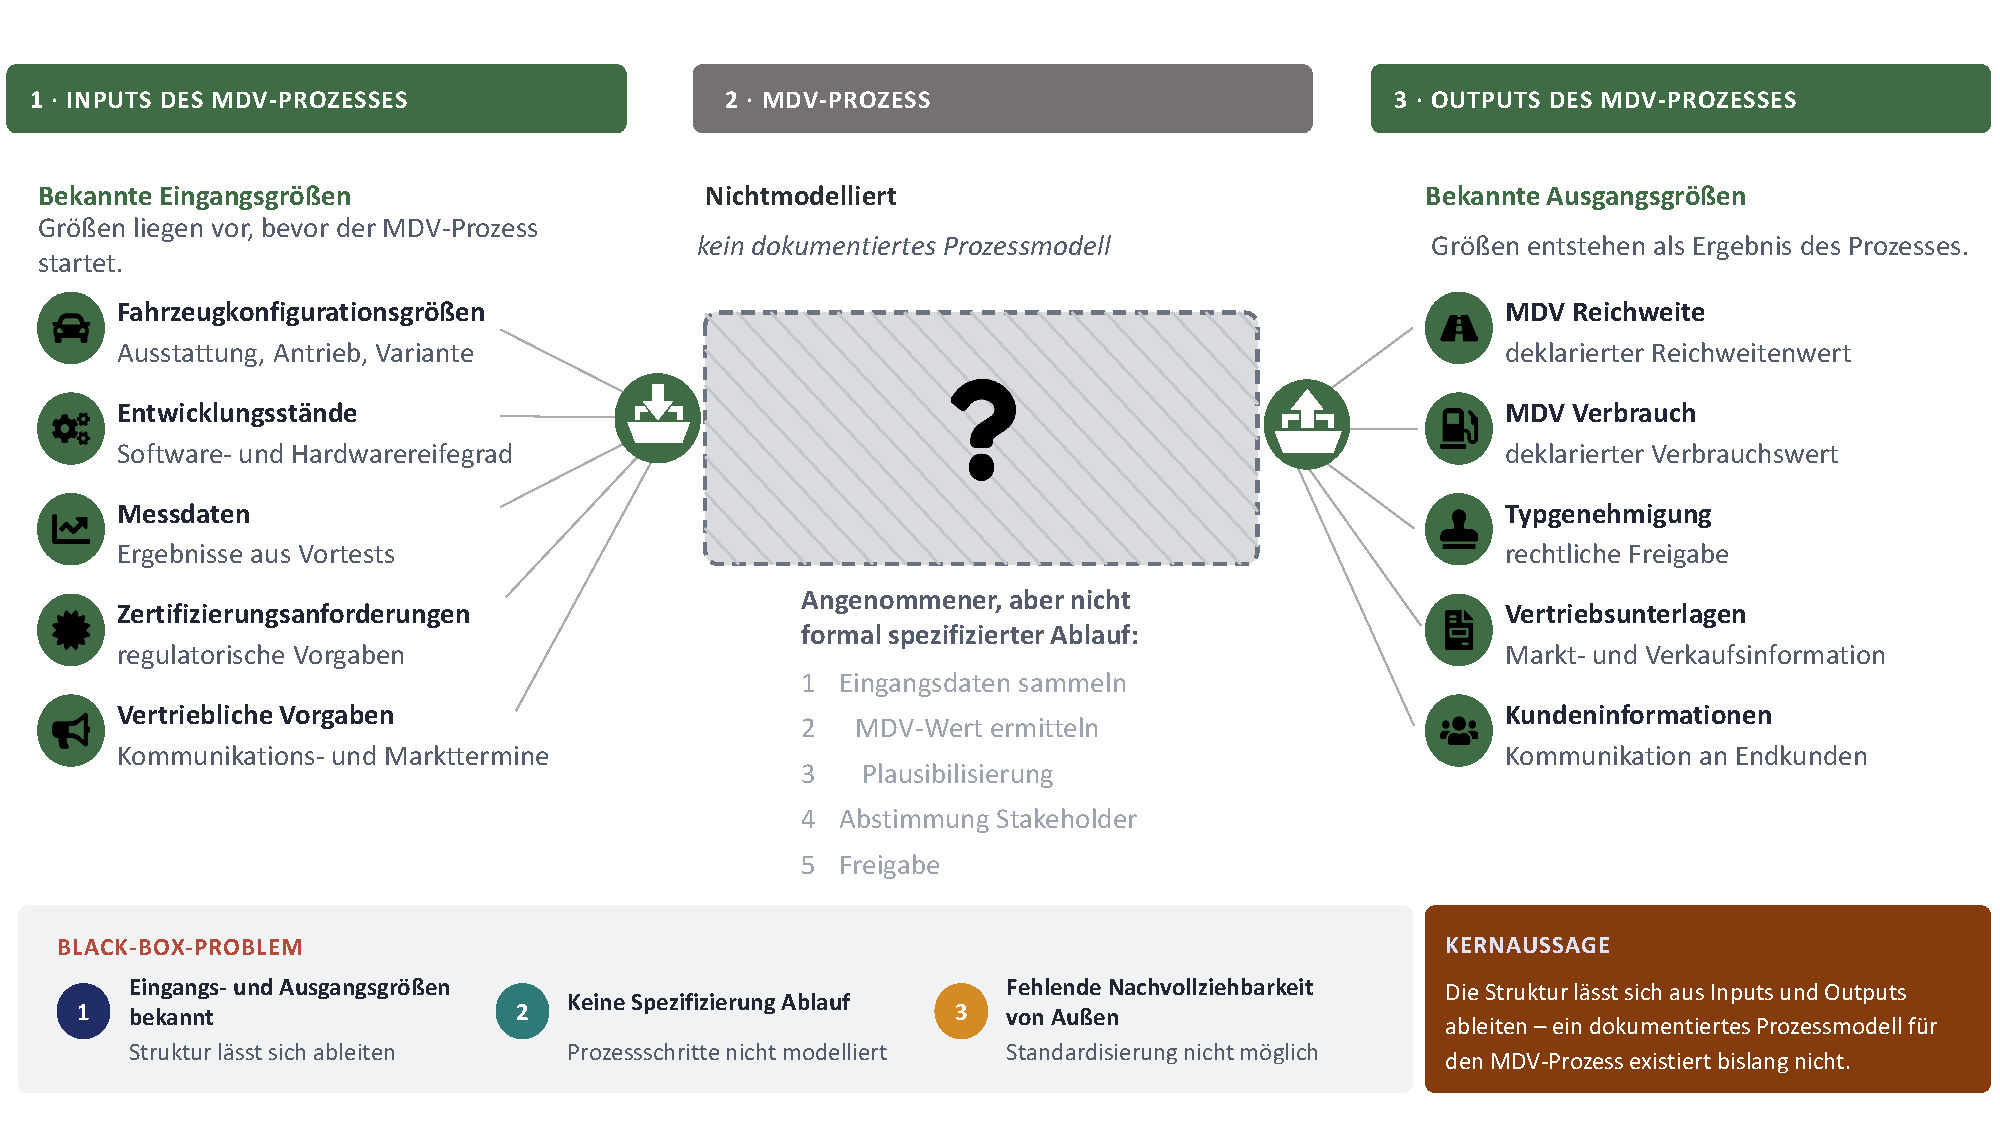
\includegraphics[width=1.0\linewidth]{images/MDV_BlackBox_Problem.pdf}
    \caption{Visualisierung des Big Picture, eigene Darstellung}
    \label{fig:bigpicture}
\end{figure}
\noindent
Das in Abbildung \ref{fig:bigpicture} dargestellte Big Picture veranschaulicht die vorliegende Problemstellung anhand der MDV-Festlegung. Die Abbildung zeigt links die bekannten Eingangsgrößen, die vor Beginn des Prozesses vorliegen. Auf der rechten Seite sind die bekannten Ausgangsgrößen abgebildet, die das Ergebnis des MDV-Ablaufs sein sollten. Das dazwischen liegende Feld wird als schraffierte Fläche dargestellt, da noch kein modelliertes Prozessmodell existiert. Die darunter angeordneten fünf Schritte sind der angenommener Ablauf, der formal nicht weiter spezifiziert wurde. Konkret umfassen die Eingangsgrößen die Fahrzeugkonfiguration, den Entwicklungsstand, vorliegende Messdaten, Zertifizierungsanforderungen sowie vertriebliche Vorgaben. Die entsprechenden Ausgangsgrößen bestehen aus dem deklarierten Reichweiten- bzw. Verbrauchswert, der Typgenehmigung, den Vertriebsunterlagen sowie den daraus abgeleiteten Kundeninformationen. Diese Gegenüberstellung zeigt, dass die Voraussetzungen und Ergebnisse des MDV-Ablaufs vorhanden sind. Die Umsetzung von Eingangs- in Ausgangsgrößen folgt jedoch keiner dokumentierten Struktur. Die im unteren Bereich der Abbildung ergänzte Zusammenfassung fasst die Kernaussage in drei Punkten zusammen. Die Struktur des Prozesses lässt sich aus den bekannten Rahmengrößen ableiten, der eigentliche Ablauf bleibt jedoch unspezifiziert. Dadurch ist eine Nachvollziehbarkeit gegenüber Prüfinstanzen sowie unternehmensinternen Stakeholdern nicht gegeben.
\\
Bei diesem Ablauf sind mehrere Fachbereiche mit jeweils eigenen Systemen und Datenbeständen beteiligt, die über die Eingangs- und Ausgangsgrößen mit dem Prozess verbunden sind. Die Herausforderung liegt nicht in den Fachbereichen selbst, sondern an der Schnittstelle zwischen ihnen und dem MDV-Ablauf sowie im Ablauf selbst. Jedem Fachbereich ist zwar bekannt, welche Größen er einbringt oder empfängt. Für die übrigen Beteiligten ist es jedoch nicht klar formal definiert welche Schritte, Verantwortlichkeiten und Entscheidungen innerhalb des Prozesses tatsächlich dazwischen liegen. Dadurch wird die Zusammenarbeit der Fachbereiche auf den reinen Austausch von Ein- und Ausgangsgrößen reduziert, ohne dass die beteiligten Parteien den dahinterliegenden Ablauf nachverfolgen können. Damit fehlt eine Grundlage für ein gemeinsames Verständnis des Prozesses und dessen Standardisierung.
\\
Neben dieser Herausforderung tragen weitere Faktoren zur Komplexität dieses Problem bei. Durch die Beteiligung mehrerer Fachbereiche mit unterschiedlichen fachlichen Blickwinkeln und Interessen erhöht sich die Anzahl aller möglichen Schnittstellen, an denen Informationslücken entstehen können. Ein weiterer Punkt ist die Heterogenität der Inputs, die aus unterschiedlichen Quellen und Systemen stammen und damit eine einheitliche Beschreibung des Prozesses erschweren. Für die verschiedenen Märkte existieren darüber hinaus jeweils eigene regulatorische Anforderungen, Zertifizierungsverfahren und Zeitschienen. Dadurch entstehen parallel mehrere marktspezifische Vorgehensweisen für die zu zertifizierenden Märkte. Eine vollständig einheitliche Ausgestaltung des Prozesses ist unter diesen Rahmenbedingungen nicht möglich, da marktspezifische Unterschiede berücksichtigt werden müssen. Daneben ist der MDV-Prozess in einen übergeordneten Rahmen eingebunden. Der \acs{WLTP}-Prozess bezeichnet bei Mercedes-AMG den internen Gesamtprozess rund um das \acs{WLTP}-Verfahren und setzt sich aus mehreren Teilprozessen der beteiligten Fachbereiche und Gewerke zusammen. Dazu gehört auch der MDV-Prozess, der innerhalb des Gesamtprozesses als Teilprozess eingebunden ist, und der derzeit an die Abgasnorm Euro 7 angepasst wird \citeintern{wltp_eu7_workshop2026}. Dementsprechend funktioniert der MDV-Prozess zwar operativ, seine innere Struktur ist von außen jedoch weder nachvollziehbar noch systematisch weiterentwickelbar. Zur Beantwortung der eingangs formulierten Forschungsfrage ist deswegen eine Methodik der Prozessaufnahme und -modellierung notwendig, mit der sich die beschriebene Black-Box-Problematik auflösen lässt. Diese Methodik wird im folgenden Kapitel vorgestellt.




%TODO




% Die Forschungsfrage nennt Prozesstransparenz. Das Fazit sagt „nachvollziehbar“ und „erstmals als gemeinsame Grundlage nach Freigabe“, prüft aber weder Entscheidungen noch Prüfinstanzen aus Kap. 2. Entscheidungen werden zu „Vorgehen“ abgeschwächt.


\chapter{Methodik}
\label{chap:methodik}
Zur Auflösung der beschriebenen Black-Box-Problematik wird im vorliegenden Kapitel die methodische Grundlage für die Aufnahme und Modellierung des MDV-Prozesses dargelegt. Zunächst wird das grundsätzliche Vorgehen der Prozessaufnahme und -modellierung beschrieben, anschließend wird BPMN 2.0 als die verwendete Notation vorgestellt. Zum Abschluss wird die Verortung des daraus resultierenden Prozessmodells im Mehrebenenmodell der Prozesslandkarte diskutiert.

\section{Vorgehensweise der Prozessaufnahme und -modellierung}

\section{BPMN 2.0 methodische Grundlage}

\section{Verortung im Mehrebenenmodell der Prozesslandkarte}
\chapter{Transfer}
\label{chap:transfer}
Im Folgendem wird die in Kapitel~\ref{chap:methodik} beschriebene Methodik auf den MDV-Prozess angewendet, um den bislang nicht modellierten Ablauf transparent darzustellen. Zuerst wird die Erstaufnahme des MDV-Ablaufs beschrieben und daraufhin die Modellierung mit BPMN 2.0 in Signavio. Danach wird das  Modell in der Prozessarchitektur eingeordnet.

\section{Erstaufnahme des MDV-Ablaufs}
\label{sec:erstaufnahme}
Gemäß Abschnitt~\ref{sec:prozessaufnahme} wurden die Prozessschritte, die Verantwortlichen sowie die Eingangs- und Ausgangsgrößen des MDV-Prozesses erhoben. Damit das Modell für alle beteiligten Fachbereiche verständlich bleibt, wurde der Ablauf in Hauptschritte mit jeweils einer Tätigkeitsbeschreibung gegliedert. Da das Prozesswissen auf einzelne Fachexperten verteilt war und kein dokumentierter Ablauf vorlag, wurden drei Interviews mit Vertretern aus drei Fachbereichen geführt, die aufgrund ihrer Beteiligung unterschiedliche Abschnitte des MDV-Prozesses abdecken konnten. Eine Einschränkung der Aufnahme bestand darin, dass die Interviews zu Beginn ausschließlich die Perspektiven einzelner Fachexperten widerspiegelten. Eine Dokumentenanalyse wurde nicht durchgeführt, da die vorhandenen Unterlagen den tatsächlichen Ablauf nicht vollständig abbildeten. Auf einen gemeinsamen Workshop wurde auch verzichtet, um die unterschiedlichen Sichtweisen der Fachbereiche getrennt zu erfassen. 
\\
Als Ergebnis der Erstaufnahme wurden 13 Prozessschritte vom Kick-off bis zur Übermittlung des finalen MDV erfasst. Um die Ergebnisse abzusichern, wurde das  entwickelte Prozessmodell gemeinsam mit den direkt Beteiligten fachlich abgestimmt. Die in Kapitel~\ref{chap:problemkontext} angenommene Abfolge diente einer ersten Strukturierung der bestehenden Black Box und wird durch den nun aufgenommenen Ablauf abgelöst. Die Durchführung liegt beim Team Konformitäts-Testing, während übrige Fachbereiche konsultiert oder informiert werden. Die beteiligten Rollen sind in Tabelle \ref{tab:rollen} aufgelistet. Als Eingangsgrößen wurden u. a. der Software-Reifegrad und der Terminplan der Zertifizierung aufgenommen. Daneben wurden drei Entscheidungspunkte erfasst, bei denen die Vollständigkeit der Ergebnisse sowie die Bestätigung des Pre-MDV und des finalen MDV geprüft werden. Die Ausgangsgröße bildet der finale MDV, der schließelich im System eingetragen und an eine weitere Abteilung übermittelt wird. 

\section{Modellierung und Beschreibung des MDV-Prozesses in Signavio}
\label{sec:modellierung}
Der MDV-Prozess wurde auf Grundlage der Ergebnisse aus Abschnitt \ref{sec:erstaufnahme} in Signavio modelliert, da unternehmensweite Prozesse bei Mercedes-AMG auf dieser Plattform abgebildet werden \citeintern{signavio2026intranet}. Die Abbildung \ref{fig:MDV-Prozess} zeigt das Modell für den Markt Westeuropa, das die 13 Prozessschritte abbildet. Weil das ursprüngliche Modell zu breit für eine lesbare Darstellung auf einer Seite ist, wird eine vereinfachte Fassung gezeigt, ohne Rollen, Datenobjekte, Systeme sowie Tätigkeitsbeschreibungen. Die Elemente der Notation aus der Abbildung \ref{fig:BPMN} wurden für den vorliegenden Prozess verwendet. Hierbei wurden die Aktivitäten einem Pool für Mercedes-AMG und einer Lane für das Team Konformitäts-Testing zugeordnet, was den Prozess durchführt. Die übrigen Fachbereiche wurden als Rollen an den Aktivitäten in Tabelle \ref{tab:rollen} hinterlegt, da bis zu elf Rollen pro Aktivität die Darstellung als Lane unübersichtlich gemacht hätten.
\newline
Der modellierte Ablauf gliedert sich in drei Phasen. Der Prozess beginnt mit dem Startereignis \glqq AZST Eintrag Zert. Vorgang abgeschlossen\grqq, sobald der Zertifizierungsvorgang im Abgas-Zertifizierungs-Steuerungstool (\acs{AZST}) eingetragen wurde. Im anschließenden Kick-off werden die Fachbereiche konsultiert und liefern den Input, aus dem die MDV-Meilensteine für den Terminplan Zertifizierung entstehen. Daraufhin prüft ein Gateway, ob alle notwendigen Ergebnisse vorliegen, wobei fehlende Informationen zunächst eingeholt werden, bevor beide Pfade wieder zusammenlaufen. Anschließend werden die Vortestergebnisse konsolidiert, wobei die Ergebnisse des Ausrollprozesses über ein UND-Gateway einfließen, und die Messwerte bewertet. Die erforderlichen Informationen werden in der Aktivität \glqq Notwendige Daten zusammengeführt\grqq gebündelt.
\newline
In der zweiten Phase wird daraufhin auf Basis der vorherigen Phase der Pre-MDV ermittelt, dessen Output der MDV-Vorschlag ist. Dieser dient als Input für die Festlegung, deren Ergebnis, der \glqq MDV inklusive \acs{CoP}-Puffer \grqq , als Zwischenereignis dargestellt wird. Nachdem der AK Zertifizierung und die Projektleitersitzung informiert wurden, prüft ein Gateway die Bestätigung, andernfalls führt der Ablauf zur Festlegung zurück.
\newline
Dementsprechend wird in der dritten Phase der finale MDV nach demselben Muster unter Einbezug der Zertifizierungsergebnisse ermittelt und festgelegt, in den Fachgremien beschlossen und bei fehlendem Beschluss erneut festgelegt. Nach der Freigabe teilt ein UND-Gateway den Ablauf in die Eintragung im \acs{AZST} und die Übermittlung an die Abteilung \glqq MO/QZE\grqq , bevor der Prozess mit dem Endereignis endet.
\newline
Um den in Abschnitt \ref{sec:erstaufnahme} festgelegten Detaillierungsgrad einzuhalten, wurde jede Aktivität mit einer Tätigkeitsbeschreibung hinterlegt. Am 23. März 2026 wurde das Prozessmodell mit den direkten Prozessbeteiligten abgestimmt und fachlich bestätigt. Damit sind die in Kapitel \ref{chap:problemkontext} angenommenen Ablaufschritte sowie die Verantwortlichkeiten erstmals in einem Prozessmodell dargestellt. Dies bildet die Grundlage für die Verortung in Abschnitt \ref{sec:verortung}.

\section{Einordnung des MDV-Modells in die Prozessarchitektur}
\label{sec:verortung}

Zunächst wurde die Ebene des MDV-Prozesses in der Prozessarchitektur bestimmt und anschließend geprüft, ob er einer der Kategorien Management-, Kern- oder Unterstützungsprozesse zugeordnet werden kann. Die Prozessarchitektur von Mercedes-AMG umfasst vier Ebenen. Der MDV-Prozess liegt auf der vierten und damit untersten Ebene \citeintern{signavio_prozesslandkarte2026}.
\newline
Die Kategorien Management-, Kern- und Unterstützungsprozesse werden in der Literatur auf der obersten Ebene der Prozessarchitektur, der Prozesslandkarte, verwendet (vgl. Abschnitt~\ref{sec:Prozesslandkarte}). Da der MDV-Prozess auf der vierten Ebene liegt, wurde er keiner dieser Kategorien eigenständig zugeordnet. Seine Einordnung erfolgt stattdessen über die Hierarchie, d. h. über den übergeordneten \acs{WLTP}-Prozess, aus dem er als Teilprozess hervorgeht  \citeintern{wltp_eu7_workshop2026}, \citeintern{signavio_prozesslandkarte2026}. Dies ist mit der Literatur vereinbar, da die Bezeichnungen nicht einheitlich definiert sind und die Einordnung je nach Organisation abweichen kann \cite{ottenlips2025geschaftsprozessmanagement}.
\newline
Die Einordnung ist vorläufig, da der WLTP-Gesamtprozess derzeit an die Abgasnorm Euro 7 angepasst wird und die Veröffentlichung in Signavio erst nach der Gremienfreigabe vorgesehen ist \citeintern{wltp_eu7_workshop2026}. Dementsprechend ist die Einordnung bei Änderungen des Gesamtprozesses erneut zu prüfen. 




% Zunächst wurde der MDV-Prozess einer Kategorie zugeordnet, anschließend seine Ebene bestimmt und abschließend seine Beziehung zu angrenzenden Prozessen betrachtet. Der MDV-Prozess wurde den Kernprozessen zugeordnet, da er sich auf das Produkt bezieht und den deklarierten Wert liefert, der für die Typgenehmigung und die Kundeninformation benötigt wird (vgl. Abschnitt~\ref{sec:Prozesslandkarte}). Eine Zuordnung zu den Unterstützungsprozessen wurde verworfen, da der Prozess den übrigen Prozessen keine Ressourcen oder Grundlagen bereitstellt, sondern einen produktbezogenen Wert liefert. Eine Zuordnung zu den Managementprozessen wurde ebenfalls verworfen, da der Prozess keine Vorgaben für andere Prozesse festlegt, sondern selbst einen konkreten Wert ermittelt. Hinsichtlich der Ebene ist der MDV-Prozess ein Teilprozess des \acs{WLTP}-Prozesses \citeintern{wltp_eu7_workshop2026}. Da seine 13 Prozessschritte in BPMN 2.0 modelliert wurden, liegt er auf der untersten Ebene der Prozessarchitektur, auf der der Ablauf eines einzelnen Prozesses im Detail abgebildet wird (vgl. Abschnitt~\ref{sec:Prozesslandkarte}). Entsprechend den Beziehungsarten aus Abschnitt~\ref{sec:Prozesslandkarte} geht der MDV-Prozess durch Zerlegung als Teilprozess aus dem \acs{WLTP}-Prozess hervor. Zu angrenzenden Prozessen steht er in einer Sequenzbeziehung, da Prozesse, die die Fahrzeuge bereitstellen und Entwicklungs-, Simulations- und Vortestergebnisse liefern, vorgelagert sind und ein Prozess, der den ermittelten MDV weiterverwendet, nachgelagert ist \citeintern{wltp_eu7_workshop2026}. Daneben bestehen durch Spezialisierung marktspezifische Varianten des Prozesses, von denen in der vorliegenden Arbeit nur der Markt Westeuropa modelliert wurde. 
\chapter{Fazit und Ausblick}
\label{chap:fazit}

Ziel war es, den bislang undokumentierten MDV-Prozess für Verbrauch und Reichweite bei Mercedes-AMG methodisch zu erfassen, mit BPMN 2.0 in Signavio zu modellieren und in die übergeordnete Prozessarchitektur einzuordnen. Hierzu wurde der Ablauf in Interviews mit Vertretern von drei Fachbereichen aufgenommen und als Modell mit 13 Prozessschritten abgebildet. Das Modell macht die Schritte, die Verantwortlichkeiten und die Entscheidungen zwischen den bekannten Eingangs- und Ausgangsgrößen sichtbar und schließt damit die in Kapitel~\ref{chap:problemkontext} beschriebene Lücke. Da es mit den direkten Prozessbeteiligten fachlich abgestimmt wurde, kann der Ablauf nun gegenüber Stakeholdern und Prüfinstanzen dargestellt werden. Bei der Einordnung wurde der MDV-Prozess keiner der Kategorien Management-, Kern- oder Unterstützungsprozess eigenständig zugeordnet, da er auf der vierten Ebene liegt. Seine Stellung ergibt sich stattdessen als Teilprozess des WLTP-Prozesses. Das bislang bei einzelnen Mitarbeitenden liegende Prozesswissen kann nach der Veröffentlichung in Signavio als gemeinsame Grundlage genutzt werden. Der MDV-Prozess lässt sich damit für Westeuropa mit BPMN 2.0 in Signavio erfassen, modellieren und in die Prozessarchitektur einordnen.
\newline
Die Ergebnisse unterliegen jedoch Grenzen. Das Modell bildet ausschließlich Westeuropa ab, da sich die Abläufe je Markt unterscheiden, sodass eine Übertragbarkeit auf weitere Märkte nicht belegt ist. Darüber hinaus beruht die Aufnahme auf Interviews mit Vertretern von drei Fachbereichen und gibt zunächst nur deren Perspektiven wieder. Diese Einschränkung wurde durch die fachliche Abstimmung des Modells verringert, jedoch nicht aufgehoben. Ob die Nachvollziehbarkeit gegenüber Prüfinstanzen gegeben ist, wurde nicht überprüft. Daneben ist die Einordnung vorläufig, da der WLTP-Gesamtprozess derzeit an Euro 7 angepasst wird (vgl. Abschnitt~\ref{sec:verortung}). Für die weitere Arbeit bietet es sich an, die Einordnung nach Abschluss der Euro-7-Anpassung und der Gremienfreigabe erneut zu prüfen und das Modell anschließend in Signavio zu veröffentlichen. Darüber hinaus sollte das Modell regelmäßig mit der Praxis abgeglichen werden, da sich Abläufe und regulatorische Anforderungen ändern.


% Add citation commands in the text where appropriate, e.g., \cite{example}
\bibliographystyle{IEEEtran}
\bibliography{references}

\bibliographystyleintern{IEEEtran}
\bibliographyintern{intern}


\end{document}

%Hinweis: \cleardoublepage \cleardoublepage
